\documentclass[11pt,table]{beamer}
\mode<presentation>
\usepackage{etex}
\usepackage{graphicx}
\usepackage{epstopdf}
\usepackage[english]{babel}
\usepackage{tabularx}
\usepackage{booktabs}
\usepackage{mathrsfs}
\usepackage{multicol}
\usepackage{bm}
\usepackage{subcaption}
\usepackage{wrapfig}
\usepackage{dcolumn}
\usepackage{threeparttable}
\usepackage{booktabs}
\usepackage{bbm}
\usepackage{amsmath,dsfont,listings}
\usepackage{amssymb}
\usepackage{rotating}
\usepackage{multirow}
\usepackage{tcolorbox}
\usepackage[authoryear]{natbib}
\usepackage{circledsteps}
\usepackage{qtree}

\usepackage{tikz}
\usetikzlibrary{arrows,decorations.pathmorphing,backgrounds,fit,positioning,shapes.symbols,chains}
\setbeamertemplate{section in toc}[sections numbered]
\setbeamertemplate{caption}[numbered]

\bibliographystyle{Econometrica}

\setbeamersize{text margin right=3.5mm, text margin left=7.5mm}  % text margin
\setbeamersize{sidebar width left=0cm, sidebar width right=0mm}
\setbeamertemplate{sidebar right}{}
\setbeamertemplate{sidebar left}{}

\definecolor{text-grey}{rgb}{0.45, 0.45, 0.45} % grey text on white background
\definecolor{bg-grey}{rgb}{0.66, 0.65, 0.60} % grey background (for white text)
\definecolor{fu-blue}{RGB}{0, 51, 102} % blue text
\definecolor{fu-green}{RGB}{153, 204, 0} % green text
\definecolor{fu-red}{RGB}{204, 0, 0} % red text (used by \alert)
\definecolor{BrewerBlue}{HTML}{377EB8} % Define Brewer Blue
\definecolor{BrewerRed}{HTML}{E41A1C}  % Define Brewer Red

\setbeamertemplate{frametitle}{%
    \vskip-30pt \color{text-grey}\large%
    \begin{minipage}[b][23pt]{\textwidth}%
    \flushleft\insertframetitle%
    \end{minipage}%
}

\setbeamertemplate{navigation symbols}{} 

%%% begin title page
\setbeamertemplate{title page}{
\vskip2pt\hfill
\vskip19pt\hskip3pt

% set the title and the author
\vskip4pt
\parbox[top][1.35cm][c]{11cm}{\LARGE\color{text-grey} \textcolor{red1}{RL}earning:\\[1ex] \inserttitle \\[1ex] \small \quad \\[3ex]}
\vskip17pt
\parbox[top][1.35cm][c]{11cm}{\small Unit 4-3: \insertsubtitle \\[2ex] \insertauthor \\[1ex]}
}
%%% end title page

%%% colors
\usecolortheme{lily}
\setbeamercolor*{normal text}{fg=black,bg=white}
\setbeamercolor*{alerted text}{fg=fu-red}
\setbeamercolor*{example text}{fg=fu-green}
\setbeamercolor*{structure}{fg=fu-blue}

\setbeamercolor*{block title}{fg=white,bg=black!50}
\setbeamercolor*{block title alerted}{fg=white,bg=black!50}
\setbeamercolor*{block title example}{fg=white,bg=black!50}

\setbeamercolor*{block body}{bg=black!10}
\setbeamercolor*{block body alerted}{bg=black!10}
\setbeamercolor*{block body example}{bg=black!10}

\setbeamercolor{bibliography entry author}{fg=fu-blue}
\setbeamercolor{bibliography entry journal}{fg=text-grey}
\setbeamercolor{item}{fg=fu-blue}
\setbeamercolor{navigation symbols}{fg=text-grey,bg=bg-grey}
%%% end colors

%%% headline
\setbeamertemplate{headline}{
\vskip30pt
}
%%% end headline

%%% footline
\newcommand{\footlinetext}{
%\insertshortinstitute, \insertshorttitle, \insertshortdate
}
\setbeamertemplate{footline}{
\vskip2pt
\hfill \raisebox{-1pt}{\usebeamertemplate***{navigation symbols}}
\hfill \insertframenumber\hspace{10pt}
\vskip4pt
}
%%% end footline

%%% settings for listings package
\lstset{extendedchars=true, showstringspaces=false, basicstyle=\footnotesize\sffamily, tabsize=2, breaklines=true, breakindent=10pt, frame=l, columns=fullflexible}
\lstset{language=Java} % this sets the syntax highlighting
\lstset{mathescape=true} % this switches on $...$ substitution in code
% enables UTF-8 in source code:
\lstset{literate={ä}{{\"a}}1 {ö}{{\"o}}1 {ü}{{\"u}}1 {Ä}{{\"A}}1 {Ö}{{\"O}}1 {Ü}{{\"U}}1 {ß}{\ss}1}
%%% end listings

\usepackage{concmath}
\usepackage{xcolor}
\definecolor{red1}{RGB}{206, 17, 38}
\definecolor{blue1}{RGB}{16, 118, 208}
\definecolor{gray1}{RGB}{117, 115, 115}
\usepackage{hyperref}


\newtheorem{proposition}{Proposition}
\newtheorem{assumption}{Definition}

\title[]{Short guides to reinforcement learning}
\subtitle[]{Deep Q-Learning}
\author[D. Rostam-Afschar]{\textcolor{gray1}{Davud Rostam-Afschar (Uni Mannheim)}}
\date[]{\today}
\subject{Econometrics}
\renewcommand{\footlinetext}{\insertshortinstitute, \insertshorttitle, \insertshortdate}
\hypersetup{
    bookmarks=false,
    unicode=false,
    pdftoolbar=false,
    pdffitwindow=true,
    pdftitle={Reinforcement Learning for Business, Economics, and Social Sciences: \insertsubtitle},
    pdfauthor={Davud Rostam-Afschar},
    pdfsubject={Reinforcement Learning},
    pdfkeywords={reinforcement learning, Deep Q-Learning},
    pdfnewwindow=true,
}
\def\sym#1{\ifmmode^{#1}\else\(^{#1}\)\fi}

\begin{document}

\begin{frame}[plain]
  \titlepage
\end{frame}

% --------------------------------------------------- Slide --
%\begin{frame}
	%\frametitle{Content}
	%\tableofcontents[]
%\end{frame}

\section{Deep Q-Networks}
{
\setbeamercolor{background canvas}{bg=BrewerBlue}
\begin{frame}
\centering
\Huge
\textcolor{white}{How to learn in very large state-action spaces?}
\thispagestyle{empty}
\end{frame}
}



\begin{frame}{Approximate Q-Learning}
\begin{figure}
	\centering
		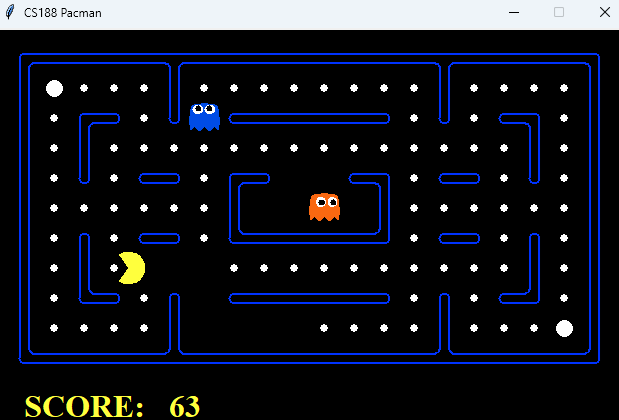
\includegraphics[width=0.90\textwidth]{figures/pacman.png}
	\label{fig:pacman}
\end{figure}

\end{frame}


\begin{frame}{Pacman as a Markov Decision Process}
\footnotesize
\begin{block}{\small Action}
\begin{itemize}
    \item Pacman's action: one of \texttt{North, South, East, West}
\end{itemize}
\end{block}
\uncover<2->{
\begin{block}{\small State Definition}
The MDP \textbf{state} is the \textit{entire game configuration} after a full ply:
\begin{itemize}
  \item Five binary flags:
    \begin{itemize}
      \item Pac-Man on field?
      \item Ghost on field?
      \item Food on field?
      \item Power-pill on field?
      \item Wall on field?
    \end{itemize}
  
  \item A ``scared ghost'' timer taking $40$ integer values $0,1,\dots,39$\\
 \uncover<3->{
   $
      2^5 \times  40 \;=\; 32 \times 40 \;=\; 1280 \text{ states per field}
    $}
		\end{itemize}
\uncover<4->{
Maze has $20 \times 11 \;=\; 220$ fields $\rightarrow$ a state is one out of $220 \times 1280 \;=\; 281,600$ configurations (many of which are impossible).
}
\end{block}
}
\only<1-4>{\vspace{13pt}}
\only<5>{Each board configuration is a separate state with separate Q-values.}
\only<6>{Pacman has no way to generalize that running into a ghost is bad for all positions.}



\end{frame}




\begin{frame}{Deep Q-Networks}


\begin{itemize}
    \item Value or Q-Function Approximation
\begin{itemize}
    \item Linear approximation
\item Neural network approximation $\rightarrow$ Deep Q-network
 
\end{itemize} 

\end{itemize}
\citep{goodfellow2016deep}    
\end{frame}

\begin{frame}{Q-function Approximation}


\begin{itemize}
    \item  Let $s=\left(x_{1}, x_{1}, \ldots, x_{n}\right)$

\item  Linear

$$Q(s, a) \approx \sum_{i} w_{a i} x_{i}$$

\item  Non-linear (e.g., neural network) 

$$Q(s, a) \approx g(\boldsymbol{x} ; \boldsymbol{w})$$ 
\end{itemize}
    
\end{frame}


\section{Gradient Q-learning}
{
\setbeamercolor{background canvas}{bg=BrewerBlue}
\begin{frame}
\centering
\Huge
\textcolor{white}{Gradient Q-learning?}
\thispagestyle{empty}
\end{frame}
}




\begin{frame}{Gradient Q-learning}


    \begin{itemize}
        \item  Minimize squared error between $Q$-value estimate and target

        \begin{itemize}
               
\item  Q-value estimate: $Q_{\textbf{w}}(s, a)$
\item  Target: $r+\gamma \max_{a \prime} Q_{\bar{w}}\left(s^{\prime}, a^{\prime}\right)$
\end{itemize}
\item  Squared error:

$$
\operatorname{Err}(\boldsymbol{\textcolor{red1}{w}})=1 / 2\left[Q_{\textcolor{red1}{w}}(s, a)-r-\gamma \max _{a^{\prime}} Q_{\overline{\boldsymbol{w}}}\left(s^{\prime}, a^{\prime}\right)\right]^{2},
$$
where $\overline{\boldsymbol{w}}$ is treated fixed.
\item  Gradient

%
%
$$
\frac{\partial E r r}{\partial \boldsymbol{w}}=\left[Q_{\boldsymbol{w}}(s, a)-r-\gamma \max _{a \prime} Q_{\overline{\boldsymbol{w}}}\left(s^{\prime}, a^{\prime}\right)\right] \frac{\partial Q_{w}(s, a)}{\partial \boldsymbol{w}}
$$ 
    \end{itemize}
\end{frame}

\begin{frame}{Gradient Q-learning}

\begin{tcolorbox}[colframe=black, boxrule=1pt, sharp corners]

\textcolor{red1}{Gradient Q-learning (s, $Q^{*}$)}

 Initialize weights $\boldsymbol{w}$ uniformly at random in [-1,1]
    
Observe current state $s$

Loop

\begin{itemize}
    \item[]  Select action $a$ and execute it
    \item[] Receive immediate reward $r$
    \item[] Observe new state $s^{\prime}$
    \item[] Gradient: $\frac{\partial E r r}{\partial \boldsymbol{w}}=\left[Q_{\boldsymbol{w}}(s, a)-r-\gamma \max _{a^{\prime}} Q_{\boldsymbol{w}}\left(s^{\prime}, a^{\prime}\right)\right] \frac{\partial Q_{\boldsymbol{w}}(s, a)}{\partial \boldsymbol{w}}$
    \item[] Update weights: $\boldsymbol{w} \leftarrow \boldsymbol{w}-\alpha \frac{\partial E r r}{\partial \boldsymbol{w}}$
    \item[] Update state: $s \leftarrow s^{\prime}$
\end{itemize}
Until convergence of $Q^{*}$

Return $Q^{*}$

\end{tcolorbox}
			
\end{frame}

\begin{frame}{Convergence of Tabular Q-learning}


   \begin{itemize}
       \item  Tabular Q-Learning converges to optimal Q-function under the following conditions:

$$
\sum_{n=0}^{\infty} \alpha_{n}\rightarrow\infty \text { and } \sum_{n=0}^{\infty}\left(\alpha_{n}\right)^{2}<\infty
$$

\item Let $\alpha_{n}(s, a)=1 / n(s, a),$

\begin{itemize}
    \item  where $n(s, a)$ is \# of times that $(s, a)$ is visited\\[2ex]
\end{itemize}
\item  Q-learning
$$Q(s, a) \leftarrow Q(s, a)+\alpha_{n}(s, a)\left[r+\gamma \max _{a^{\prime}} Q\left(s^{\prime}, a^{\prime}\right)-Q(s, a)\right]$$ 
   \end{itemize} 
\end{frame}


\begin{frame}{Convergence of  Linear Gradient Q-Learning}


\begin{itemize}
    \item  Linear Q-Learning converges under the same conditions:

$$
\sum_{n=0}^{\infty} \alpha_{n}\rightarrow\infty \text { and } \sum_{n=0}^{\infty}\left(\alpha_{n}\right)^{2}<\infty
$$

\item Let $\alpha_{n}=1 / n$

\item  Let $Q_{w}(s, a)=\sum_{i} w_{i} x_{i}$

\item  Q-learning
$$
\boldsymbol{w} \leftarrow \boldsymbol{w}-\alpha_{n}\left[Q_{\boldsymbol{w}}(s, a)-r-\gamma \max _{a^{\prime}} Q_{\boldsymbol{w}}\left(s^{\prime}, a^{\prime}\right)\right] \frac{\partial Q_{\boldsymbol{w}}(s, a)}{\partial \boldsymbol{w}}
$$ 
\end{itemize}
    
\end{frame}



\begin{frame}{Divergence of Non-linear Gradient Q-learning}


    \begin{itemize}
        \item Even when the following conditions hold

$$
\sum_{n=0}^{\infty} \alpha_{n}\rightarrow\infty \text { and } \sum_{n=0}^{\infty}\left(\alpha_{n}\right)^{2}<\infty
$$

 non-linear Q-learning may diverge

\item Intuition:

 \begin{itemize}
     \item Adjusting $\boldsymbol{w}$ to increase $Q$ at $(s, a)$ might introduce errors 
 \end{itemize}
    \end{itemize}
\end{frame}

\begin{frame}{Mitigating divergence}

Two tricks are often used in practice:\\[2ex]
 \begin{enumerate}
\item Experience replay\\[2ex]
\item Use two networks:
 \begin{itemize}
\item Q-network
\item Target network
 
 \end{itemize}
 
 \end{enumerate}
\end{frame}


\section{Experience Replay}
{
\setbeamercolor{background canvas}{bg=BrewerBlue}
\begin{frame}
\centering
\Huge
\textcolor{white}{Experience Replay}
\thispagestyle{empty}
\end{frame}
}


\begin{frame}{Experience Replay}
\begin{figure}
	\centering
		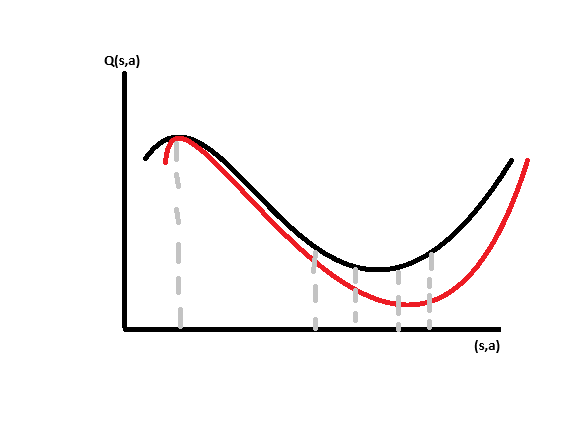
\includegraphics[width=1\textwidth]{figures/replay.png}
	\label{fig:replay}
\end{figure}

\end{frame}

\begin{frame}{Experience Replay}


\begin{itemize}
    \item Idea: store previous experiences $(s,a,s',r)$ into  a buffer and sample a mini-batch of previous experiences at each step to learn by Q-learning\\[2ex]

 \item Advantages
\begin{itemize}
    \item Break correlations between successive updates (more stable learning)
	\item Fewer interactions with environment needed to converge\\ (greater data efficiency)
 
\end{itemize} 
\end{itemize}
    
\end{frame}


\section{Target Network}
{
\setbeamercolor{background canvas}{bg=BrewerBlue}
\begin{frame}
\centering
\Huge
\textcolor{white}{Target Network}
\thispagestyle{empty}
\end{frame}
}

\begin{frame}{Target Network}


    \begin{itemize}
        \item Idea: Use a separate target network that is updated only periodically\\[2ex]
				repeat for each $(s,a,s',r)$  in mini-batch:

$$
\boldsymbol{w} \leftarrow \boldsymbol{w}-\alpha_{n}\left[\underbrace{Q_{\boldsymbol{w}}(s, a)}_{update}-r-\gamma \max _{a^{\prime}} \underbrace{\textcolor{red1}{Q_{\bar{w}}\left(s^{\prime}, a^{\prime}\right)}}_{\textcolor{red1}{target}}\right] \frac{\partial Q_{\boldsymbol{w}}(s, a)}{\partial \boldsymbol{w}}
$$

$\overline{\boldsymbol{w}} \leftarrow \boldsymbol{w}$

 \item Advantage: mitigate divergence 
\uncover<2>{
        \item Similar to value iteration:

repeat for all $s$

$$
\begin{aligned}
& \quad \underbrace{V(s)}_{update} \leftarrow \max _{a} R(s)+\gamma \sum_{s^{\prime}} \mathbb{P}\left(s^{\prime} \mid s, a\right) \underbrace{\bar{V}\left(s^{\prime}\right)}_{target} \forall s \\
& \bar{V} \leftarrow V
\end{aligned}
$$

\item Q-learning is a sampling version of value iteration
}
    \end{itemize}
    
\end{frame}


\begin{frame}{Deep Q-network}

Google Deep Mind:\\[2ex]
\begin{itemize}
\item Deep Q-network: Gradient Q-learning with

 \begin{itemize}
     \item Deep neural networks
\item Experience replay
\item Target network\\[2ex]
 
 \end{itemize}
 \item Breakthrough: human-level play in many Atari  video games
 
\end{itemize}
    
\end{frame}

\begin{frame}{Deep Q-network}
\begin{tcolorbox}[colframe=black, boxrule=1pt, sharp corners]

\textcolor{red1}{DQNetwork ($Q_{\boldsymbol{w}}(s,a)$)}

Initialize weights $\boldsymbol{w}$ and $\overline{\boldsymbol{w}}$ at random in $[-1,1]$

Observe current state $s$

\quad Loop

\qquad Select action $a$ and execute it

\qquad Receive immediate reward $r$

\qquad Observe new state $s^{\prime}$

\qquad Add $\left(s, a, s^{\prime}, r\right)$ to \textcolor{red1}{experience buffer}

\qquad Update Q-func by sampling mini-batch from buffer

\qquad For each experience ($\hat{s}, \hat{a}, \hat{s}^{\prime}, \hat{r}$) in mini-batch

\quad\qquad Gradient: $\frac{\partial E r r}{\partial \boldsymbol{w}}=\left[Q_{\boldsymbol{w}}(\hat{s}, \hat{a})-\hat{r}-\gamma \max _{\widehat{a} \prime} Q_{\overline{\boldsymbol{w}}}\left(\hat{s}^{\prime}, \hat{a}^{\prime}\right)\right] \frac{\partial Q_{\boldsymbol{w}}(\hat{s}, \hat{a})}{\partial \boldsymbol{w}}$

\quad\qquad Update weights: $\boldsymbol{w} \leftarrow \boldsymbol{w}-\alpha \frac{\partial E r r}{\partial \boldsymbol{w}}$

\qquad Update state: $s \leftarrow s^{\prime}$

\qquad Every $c$ steps, update \textcolor{red1}{target}: \textcolor{red1}{$\overline{\boldsymbol{w}} \leftarrow \boldsymbol{w}$}

    \end{tcolorbox}
\end{frame}




\begin{frame}{Deep Q-Network for Atari}
    \begin{center}
        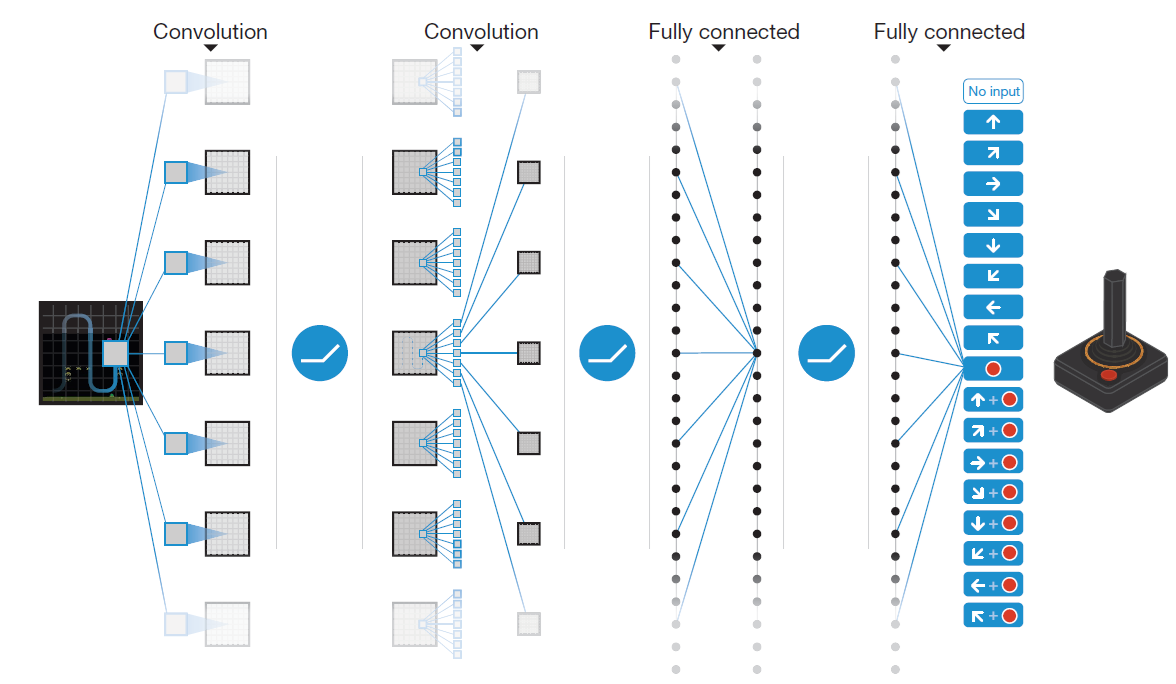
\includegraphics[width=1\textwidth]{figures/17.png}
    \end{center}
\medskip
\hfill \footnotesize\textit{Source: Mnih et al. (2015)}
\end{frame}

\begin{frame}{DQN versus Linear approx.}
   \begin{center}
        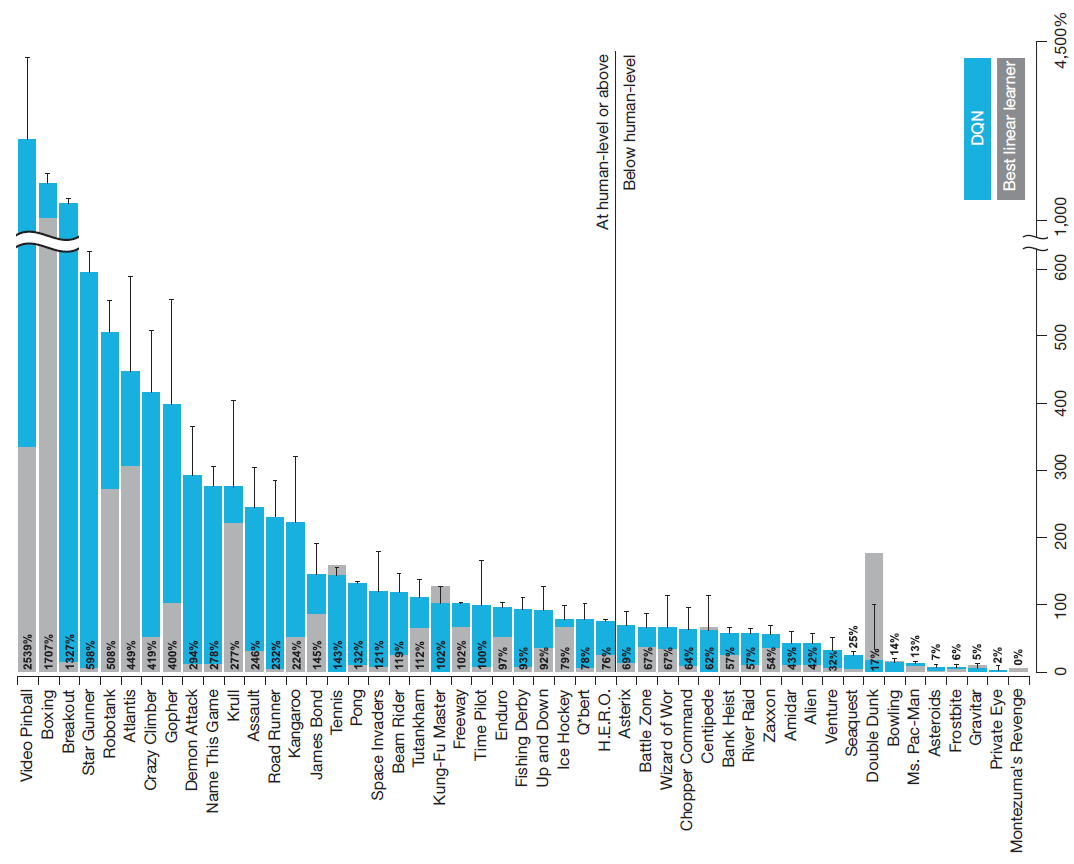
\includegraphics[width=0.75\textwidth]{figures/18.png}
    \end{center} 
\medskip
\hfill\footnotesize Note: Human: 75\% of professional human games tester. \textit{Source: Mnih et al. (2015)}
\end{frame}


\begin{frame}[t,allowframebreaks
]%\nocite{*}
\frametitle{References}
\small
\bibliography{bib}
\end{frame}
\section{Takeaways}
{
\setbeamercolor{background canvas}{bg=BrewerBlue}
\begin{frame}
\centering
\Huge
\textcolor{white}{Takeaways}
\thispagestyle{empty}
\end{frame}
}

\begin{frame}{Deep Q-Learning (DQN)}
\begin{itemize}
   \item Combines Q-learning with deep neural networks for large state-action spaces
    \item It approximates Q-values by minimizing the Bellman error using gradient descent
    \item Experience replay and target networks stabilize training and prevent divergence
    \item DeepMind's DQN achieved human-level performance on Atari games with these techniques
\end{itemize}
\end{frame}


\end{document}
